Dla tego zbioru danych osiągane są najlepsze wyniki spośród wszystkich poprzednich zbiorów.
Można zaobserwować bardzo podobne trendy zmiany wartości miar w zależności od liczby podzbiorów
kroswalidacyjnych -- w 3 osiągają lokalne minimum, następnie do 5 szybko rosną do wartości rzędu 80\%-90\%,
po czym do 9 w miarę utrzymują podobny poziom.

Mimo wstępnych obserwacji z analizy rozkładów wartości atrybutów, gdzie zauważono
potencjał zbioru danych do przetworzenia wielomianowym klasyfikatorem, okazuje się jednak
że najlepsze wyniki osiągnął klasyfikator Gaussowski.

\begin{figure}[H]
\center
    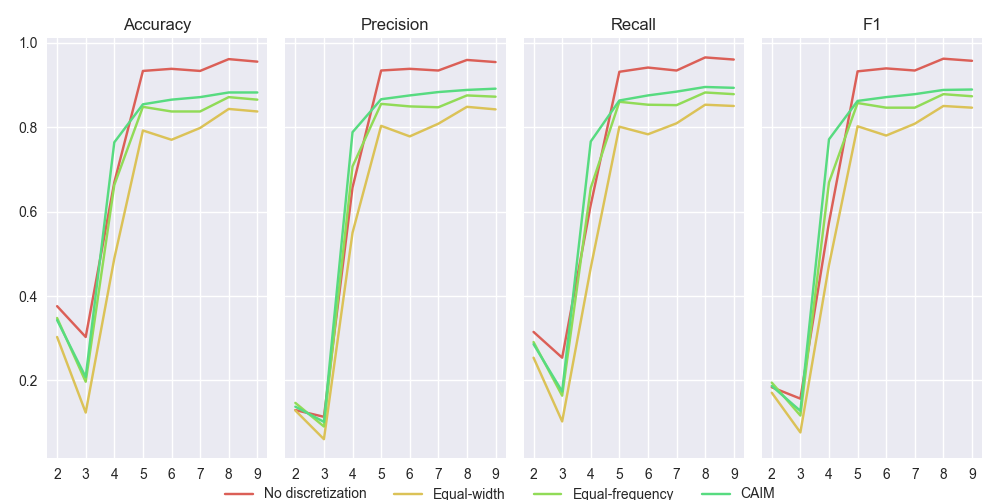
\includegraphics[width=\textwidth]{img/cv_scores_kfold/scoring_kfold_wine.png}
    \caption{Wykresy wartości metryk dla zbioru "Wine" -- kroswalidacja zwykła.}
\end{figure}

Macierz konfuzji została wybrana dla $K = 8$ i prezentuje świetne wyniki. Prawidłowe
klasyfikacje są na poziomie 93\%-100\%, a błędy są szczątkowe.

\begin{figure}[H]
\center
    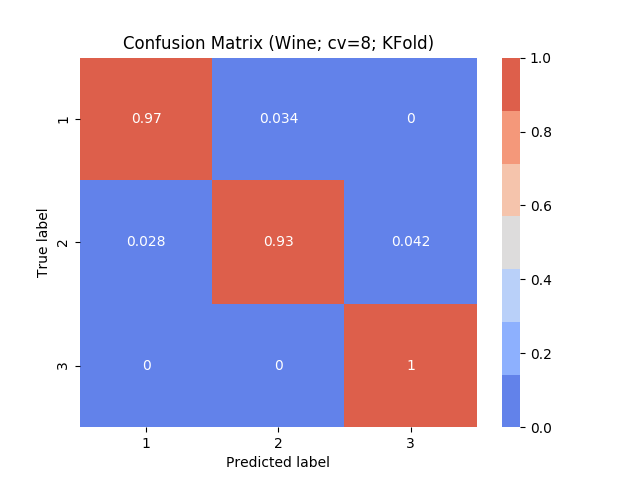
\includegraphics[width=0.6\textwidth]{img/conf_matrices/cm_Wine_cv8_KFold.png}
    \caption{Macierz konfuzji dla najlepszej wartości F1 -- kroswalidacja zwykła.}
\end{figure}

    \begin{table}[H]
        \center
        \caption{Wartości metryk dla zbioru "Wine" -- kroswalidacja zwykła.}
        \begin{tabular}{|c|c|c|c|c|c|c|c|c|c|}
            \hline
            \multirow{2}{*}{\textbf{Metoda dyskr.}} & \multirow{2}{*}{\textbf{Metryka}} & \multicolumn{8}{|c|}{\textbf{CV}} \\ \cline{3-10}
                            &  & 2 & 3 & 4 & 5 & 6 & 7 & 8 & 9 \\ \hline
            \multirow{4}{*}{\textit{Brak}}  & Accuracy & 0.376 & 0.303 & 0.669 & 0.933 & 0.938 & 0.933 & 0.961 & 0.955 \\ \cline{2-10}
                                             & Precision & 0.13 & 0.114 & 0.657 & 0.934 & 0.938 & 0.934 & 0.959 & 0.954 \\ \cline{2-10}
                                             & Recall & 0.315 & 0.254 & 0.616 & 0.931 & 0.941 & 0.934 & 0.965 & 0.96 \\ \cline{2-10}
                                             & F1 & 0.184 & 0.157 & 0.574 & 0.932 & 0.939 & 0.934 & 0.962 & 0.957 \\ \hline \hline


                                            \multirow{4}{*}{\textit{Equal-width}}  & Accuracy & 0.303 & 0.124 & 0.489 & 0.792 & 0.77 & 0.798 & 0.843 & 0.837 \\ \cline{2-10}
                                             & Precision & 0.129 & 0.061 & 0.55 & 0.803 & 0.778 & 0.808 & 0.848 & 0.842 \\ \cline{2-10}
                                             & Recall & 0.254 & 0.103 & 0.467 & 0.801 & 0.783 & 0.809 & 0.853 & 0.85 \\ \cline{2-10}
                                             & F1 & 0.171 & 0.077 & 0.473 & 0.802 & 0.78 & 0.808 & 0.85 & 0.846 \\ \hline \hline


                                            \multirow{4}{*}{\textit{Equal-freq}}  & Accuracy & 0.348 & 0.197 & 0.663 & 0.848 & 0.837 & 0.837 & 0.871 & 0.865 \\ \cline{2-10}
                                             & Precision & 0.147 & 0.091 & 0.707 & 0.855 & 0.849 & 0.847 & 0.875 & 0.872 \\ \cline{2-10}
                                             & Recall & 0.291 & 0.164 & 0.656 & 0.86 & 0.853 & 0.852 & 0.882 & 0.878 \\ \cline{2-10}
                                             & F1 & 0.195 & 0.117 & 0.669 & 0.857 & 0.846 & 0.846 & 0.878 & 0.873 \\ \hline \hline


                                            \multirow{4}{*}{\textit{CAIM}}  & Accuracy & 0.343 & 0.208 & 0.764 & 0.854 & 0.865 & 0.871 & 0.882 & 0.882 \\ \cline{2-10}
                                             & Precision & 0.138 & 0.102 & 0.788 & 0.866 & 0.875 & 0.883 & 0.888 & 0.891 \\ \cline{2-10}
                                             & Recall & 0.286 & 0.174 & 0.766 & 0.863 & 0.875 & 0.884 & 0.895 & 0.893 \\ \cline{2-10}
                                             & F1 & 0.187 & 0.128 & 0.771 & 0.862 & 0.871 & 0.878 & 0.888 & 0.889 \\ \hline \hline

            \hline
        \end{tabular}
    \end{table}

